This chapter is devoted to describing the outcomes of the preliminary research focusing on the similar already existing projects and technologies that could be utilized.
In section \ref{txt:similar_projects} the similar projects will be described together with their relations to our project and their advantages and disadvantages.
Software development methodology is described in section \ref{sec:methodology}.
Then in the section \ref{txt:development technologies} the development technologies and collaboration tools will be presented with outcome of the overall research.

%%%%%%%%%%%%%%%%%%%%%%%%%%%%%%%%%%%%%%%%%%%%%%%%%%%%%%%%%%%%%%%%%%%%%%%%%%%%%%%%%%%%%%%%%%%%%%%%%%%%
%%%%%%%%%%%%%%%%%%%%%%%%%%%%%%%%%%%%%%%%%%%%%%%%%%%%%%%%%%%%%%%%%%%%%%%%%%%%%%%%%%%%%%%%%%%%%%%%%%%%

\section{Similar projects} \label{txt:similar_projects}
No other services using exactly the same technical solution as compared to our product was found.
Nevertheless a few similar entertainment services that aim to amuse the music concert audience already exist. 
These services basically encourage the audience to use either their smartphones or other device as the source of light that helps to create impressive and colorful show.

%==================================================================================================%

\subsection{Wham City Lights}

\subsubsection{Description}
The Wham City Lights is the mobile application developed by the one year old Baltimore based start-up \footnote{\url{http://whamcitylights.com/}}. 
As far as the Digital Lighter is concerned the Wham City Light service seems to be the closest solution as it works with the users' smartphones and uses them as a source of the light and even the sound.

Users attending the given concert only need to download and install the free application, start it and then hold their smartphones in the air.
The application then controls the color displayed on the smartphone screen, the camera flashes and the sound going out of the speakers and it creates the spatial soundscapes and lighting designs.
What is more the application does not require the network connection as the instructions are modulated into the ultrasonic inaudible signal that is being continuously transmitted during the performance.

Using this innovative technique all the smartphones can be effectively synchronized so that the  changing lights and imagery on the phone follows and complete the music performance.
Nevertheless the so-called light show must be pre-programmed and this system cannot determine the location of the mobile devices.

The demonstration of the real world performance of the application and the concept for that matter can be seen in the official Wham City Lights marketing video\footnote{\url{http://www.youtube.com/watch?v=faJ1Av5kBCE}}.

\begin{figure}[!ht]
	\centering
		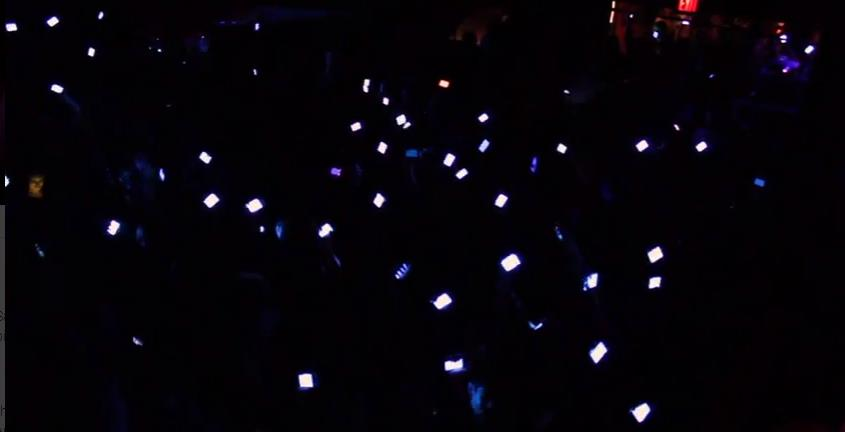
\includegraphics[width=10cm]{preliminaryStudies/wham_city_lights.jpg}
	\caption{Wham City Lights}
	\label{fig:wham_city_lights}
\end{figure}

\subsubsection{Impact}
The Wham City Lights application or its derivatives have been so far used on relatively many music events of greater importance where several thousands of people were present and used the application. To list a few:
\begin{itemize}
\item America's Got Talent 2013
\item CMA Music Festival 2013
\item Intel sales conference 2013
\item Billboard Music Awards 2013
\end{itemize}

\subsubsection{Availability}
The application is available for the devices using Android or iOS operating systems and it can be downloaded from the Google Play\footnote{https://play.google.com/store/apps/details?id=com.whamcitylights} and App Store\footnote{https://itunes.apple.com/us/app/wham-city-lights/id580034697?mt=8} respectively. The developer nevertheless offers the customers a concert specific applications with relevant user interface built-in. As for the light show itself, programming part can be done either by the customer or the developer.

\subsubsection{Relation to our project}
Like our project the Wham City Lights application builds upon users' smartphones that are remotely controlled in order to display intended imagery. 

\paragraph{Advantages}
The devices attending the light show do not need the network connection and the displayed imagery is well synchronized with the music.

\paragraph{Disadvantages}
The location of the mobile devices cannot be determined and the different processing speed of the devices causes incorrect synchronization.


\subsection{Xylobands}

\subsubsection{Description}
So called Xyloband\footnote{http://xylobands.com/} is the invention of the company RB Concepts Limited. The device itself consists of the plastic bracelet that includes the LED diodes of the different colors and the microcontroller. 
The bracelets are controlled by the radio signal being broadcast from the stage and as a result they change their colors, flashes and in general create colorful imagery.

\begin{figure}[!t]
	\centering
		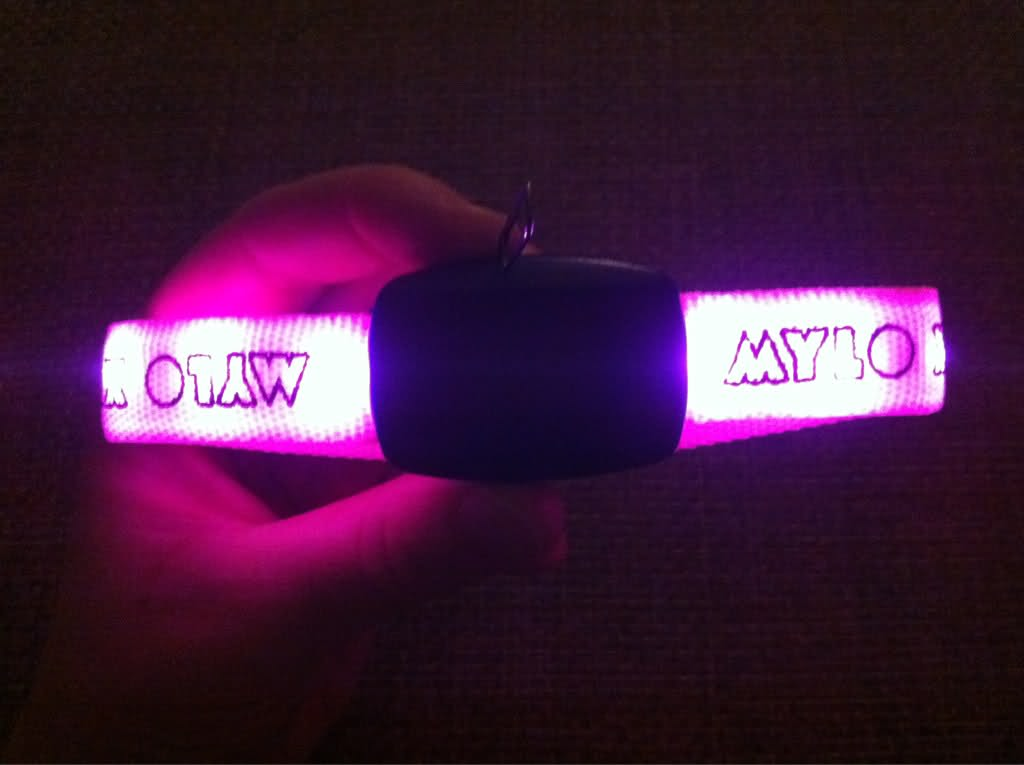
\includegraphics[width=10cm]{preliminaryStudies/xylo.jpg}
	\caption{Wham City Lights}
	\label{fig:xylo}
\end{figure}

\subsubsection{Impact}
Xylobands received great fame thanks to the well known British rock band ColdPlay which used them during their 2012 tour.

\subsubsection{Availability}
The bracelets can be ordered on the official Xylobands website.

\subsubsection{Relation to our project}
The Xylobands product is somewhat different from the Digital Lighter as it does not utilize the users' mobile devices. 
The similarity can be found in the way the bracelets are synchronized using wireless signal. 

\paragraph{Advantages}
The users do not need to bring their own mobile device and all of the audience has the possibility to become the part of the light show.

\paragraph{Disadvantages}
The location of the single participants cannot be determined.

%\section{Existing technologies and frameworks}
%\section{Evaluation of alternative solutions}

%%%%%%%%%%%%%%%%%%%%%%%%%%%%%%%%%%%%%%%%%%%%%%%%%%%%%%%%%%%%%%%%%%%%%%%%%%%%%%%%%%%%%%%%%%%%%%%%%%%%
%%%%%%%%%%%%%%%%%%%%%%%%%%%%%%%%%%%%%%%%%%%%%%%%%%%%%%%%%%%%%%%%%%%%%%%%%%%%%%%%%%%%%%%%%%%%%%%%%%%%
\section{Software development methodology}
A software development methodology is a framework used for structuring, planning and controlling the process of developing an information systems \cite{selectingMethodology}. In the real world ICT companies utilize quite a few various software development methodologies that differ mainly in the overall size of the project they are meant to manage, life cycle phases design and the level of certainty that initial requirements would not change.

One can basically choose between two main general approaches, the traditional software development process or iterative-development process \cite{fairley2009managing}. The first technique mentioned mainly comprise of so called waterfall based models. In theory the waterfall model thoroughly describes the software life cycle phases as a strict sequence that should result in a functional product. The real world experiences however show that this model is not suitable for the projects where the requirements are unclear in the preliminary phases and likely to change a lot during the development process \cite{john2011software}.

It is impossible to have the crystal clear image of the resulting product in the beginning\cite{fairley2009managing} which applies to Digital Lighter project very well. This fact prevents both the customer and the development team to specify all of the requirements beforehand. On the contrary, the team agreed with the customer it is more desirable to employ the methodology which enables the development team to add the new features in an iterative manner and to present functional pieces of code (prototypes) to the customer regularly so that the right course of the project can be maintained.

Therefore it is more reasonable to rely on the approaches from the latter group, the approaches based on iterative-development process. In general these models are designed in the way that they enable the development team to continuously verify and validate the product and detect the process problems early and as discussed with the customer this is something both development team and the customer will benefit from. It has been decided to use the agile development models as described in section \ref{txt:agile_methodologies} and specifically the Scrum model covered in section \ref{txt:scrum}.

%==================================================================================================%
\subsection{Agile methodologies} \label{txt:agile_methodologies}
Agile methodologies were created as the contrary to the traditional software development techniques based on the waterfall model. According to the Agile Manifesto \cite{agileManifesto} created by the well established non profit organization Agile Alliance\footnote{\url{http://www.agilealliance.org/}} the agile approach basically mainly focus on team-customer communication, working software, tight collaboration and ability to respond to changes. As stated in table \ref{tab:agile_vs_waterfall} these and other features agile methodologies provide suite the Digital Lighter the best as the customer stated he requires to be closely involved in the development process.

\begin{table}[htb]
	\begin{center}
	\caption{Confrontation between the agile and waterfall methodologies and their applicability in Digital Lighter project}
	\label{tab:agile_vs_waterfall}
	\def\arraystretch{1.3}
		\begin{tabularx}{0.9\textwidth}{ X c c }
		\toprule[0.5mm]
		\textbf{Digital Lighter properties} & \textbf{Agile methodologies} & \textbf{Waterfall} \\
		\midrule[0.5mm]
		Small sized team 								& \tick  & \tick 	\\
		Quick development				 				& \tick  & \cross 	\\
		Prototyping										& \tick  & \cross 	\\
		Frequent product releases 						& \tick  & \cross 	\\
		Strong customer involvement 					& \tick  & \cross 	\\
		Focus on documentation 							& \cross & \tick  	\\
		\bottomrule[0.5mm]
		\end{tabularx}
	\end{center}
\end{table}

It can be noticed that the Digital Lighter project requires the team to make a great effort writing the documentation which does not particularly correspond with the agile approach. The issue is that this is still the school project and the extensive documentation is a part of the task. Still as far as the properties of the Digital Lighter project are concerned the advantages of the agile approach are prevailing.

%==================================================================================================%
\subsection{Scrum} \label{txt:scrum}
Scrum is one of the well established agile methodologies and it has been embraced by the team for several reasons. The customer had good experience using Scrum before and he strongly encouraged the team to use this methodology. Moreover one of the team members has the real world experience working in Scrum. Even though it requires "learning-by-doing" approach to learn Scrum in this case all of the  team members were committed to learn new methodology as it seems to be widely used in the commercial field and therefore the team members would get the valuable experience.

It must be mentioned the team does not use the pure Scrum methodology but rather adjusts it to its specific needs as we are not able to fulfill all of the procedures Scrum dictates. This approach is referred to as a \textit{Scrumbut} \cite{viscardi2013professional} which comes from the self explanatory claim "We use scrum, but ...".  The Scrum framework consists of the roles, processes and artifacts \cite{viscardi2013professional}. Our approach to the role assigning and fulfilling the processes is described in section \ref{txt:utilizing_scrum}. The overall concept of Scrum can be seen on figure \ref{fig:scrum}.

\begin{figure}[hbt]
\centering
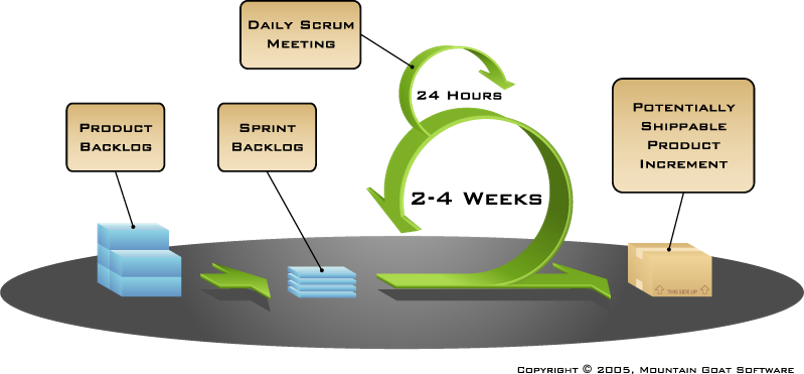
\includegraphics[width=\textwidth]{preliminaryStudies/scrum.png}
\caption{Scrum}
\label{fig:scrum}
\end{figure}

\subsubsection{Scrum related terms}

\paragraph{User story}
is a short text of user's language of a system that describes user's interaction with the system. User stories are actually narrative texts that describe an interaction of the user and the system, focusing on the value a user gains from the system.

\paragraph{Epic}
is a large \emph{user story} that will need to be broken down into smaller stories. It is too big to fit into a sprint, or it is unknown as to whether it is too big to fit into a sprint or not.

\paragraph{Task}
If user story is too complex, it can be divided into several tasks. 
Task is then basic unit of problem division.

\paragraph{Milestone} is an event that receives special attention. It can add significant value to project scheduling by helping team to more accurately determine whether or not the project is on schedule.


%%%%%%%%%%%%%%%%%%%%%%%%%%%%%%%%%%%%%%%%%%%%%%%%%%%%%%%%%%%%%%%%%%%%%%%%%%%%%%%%%%%%%%%%%%%%%%%%%%%%
%%%%%%%%%%%%%%%%%%%%%%%%%%%%%%%%%%%%%%%%%%%%%%%%%%%%%%%%%%%%%%%%%%%%%%%%%%%%%%%%%%%%%%%%%%%%%%%%%%%%
\section{Development technologies} \label{txt:development technologies}

According to the customer's requirements the product must be executable on the mobile devices and it should utilize the image processing technologies as well. Therefore we had to make two main decisions - which mobile platform to prefer and which existing image processing libraries to use. Both of the decisions are explained in greater detail in sections \ref{txt:mobile_platform} and \ref{txt:image_processing_library}.

%==================================================================================================%

\subsection{Android} \label{txt:mobile_platform}

The mobile devices market is currently flooded with smartphones and tablets running on dozen of different platforms. 
But since we try to aim the application on as many users as possible the choice was relatively straightforward.
Considering the survey carried on by the well established analyst, the company IDC, as of Q2 2013 Google's Android OS held almost 80 \% of the market share\footnote{\url{http://www.idc.com/getdoc.jsp?containerId=prUS24257413}} leaving iOS, windows Phone, BlackBerry and others well behind.
What is more all of the members of our team posses the Android based smartphone thus we decided to choose the Android platform.

\subsubsection{Android SDK}

Google provides the Android developers with all the necessary tools and API's through the open source and free SDK\footnote{Software Development Kit}. While developing under SDK the Java programming language together with the Android event-driven architecture is used.

\subsubsection{Android NDK}

Through the NDK\footnote{Native Development Kit} Google provides the toolset allowing the programmers parts of the application using native-code languages such as C and C++.
We discussed using NDK just for the computationally demanding modules such as the image processing since the applications based on already compiled code tend to run faster.
Nevertheless we are allowed to scale the problem down and thus the use of Java perfectly suffices fr our purposes.
Should the customer require to scale the problem up we can switch to using NDK anytime.

%==================================================================================================%

\subsection{OpenCV} \label{txt:image_processing_library}

As far as the image processing is considered the outcome of our preliminary research is as follows.
Currently there exist a few open source and free libraries generally focusing on working with the multimedia.
OpenCV library is probably the most well-known library providing a broad range of image processing functions.
It is written and meant to be used in conjunction with C++ but the possibility to use Java already exists too.
The support for using OpenCV on Android platform is provided through the OpenCV4Android SDK that can be obtained from the official OpenCV website\footnote{\url{http://docs.opencv.org/}} and used for free.
So far we consider this toolkit to be sufficient for our needs but should we come across any problems we might be forced to switch to the combination of OpenCV, C++ and Android NDK.

%==================================================================================================%

\subsection{TestFlight}

TestFlight\footnote{\url{https://testflightapp.com/}} is a free web service for mobile developers that provides the tools to easily deploy and distribute the mobile application. What is more TestFlight offers the SDK for developers so that it can be integrated directly into the applications. The advantage of using the TestFlight is the fact that the developer is able to track the bugs, crashes and users' or testers' feedback. The customer suggested the team to use such a service and we had to choose between the TestFlight and similar service called HockeyApp. Unlike HockeyApp the TestFlight is a free service therefore we decided to adopt this service.

%%%%%%%%%%%%%%%%%%%%%%%%%%%%%%%%%%%%%%%%%%%%%%%%%%%%%%%%%%%%%%%%%%%%%%%%%%%%%%%%%%%%%%%%%%%%%%%%%%%%
%%%%%%%%%%%%%%%%%%%%%%%%%%%%%%%%%%%%%%%%%%%%%%%%%%%%%%%%%%%%%%%%%%%%%%%%%%%%%%%%%%%%%%%%%%%%%%%%%%%%

\section{Project management tools}
Since we use Scrum methodology, we were in need to find an appropriate management tool supporting Scrum. 
There exist many possible tools, but most of them are charged from
certain number of team members. 
Here are presented tools we have used for a testing purposes or in real development.

%==================================================================================================%

\subsection{Trello}
\label{TrelloToolDescription}
Trello is a collaboration tool\footnote{\url{https://trello.com/}} that can organize tasks into various boards, it shows what task has been assigned to who and in what stage the task is.
Even though Trello supports a lot of features, it is not originally designed for Scrum use and there is no support of \emph{Epics}, \emph{Burn-down chart} and time tracking. Therefore after short discussion we have decided that Trello is not suitable for our purpose.

%==================================================================================================%

\subsection{Gravity} 
\label{GravityToolDescription}
Gravity is a simple project management tool\footnote{\url{www.gravitydev.com}} currently in beta phase.
It supports splitting stories into tasks and also automatically calculates \emph{Burn-down chart}. 
Last but not least it supports it is free of charge for 5 team members, it supports issue tracking and support labels, which can be used for \emph{Epics}.
On the other hand it does not support time tracking.
You can see picture of Gravity's features in image \ref{img:gravity}. After a while it showed up that Gravity has some bugs since it is in Beta version and also it misses a time tracking feature.

\begin{figure}[!h]
	\centering
		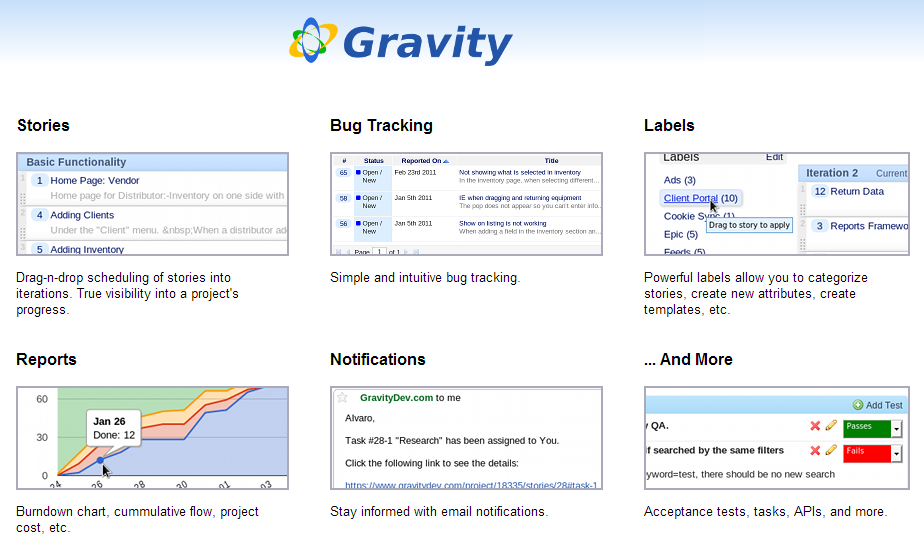
\includegraphics[width=11cm]{preliminaryStudies/gravity.png}
	\caption{Gravity features}
	\label{img:gravity}
\end{figure}
%==================================================================================================%

\subsection{Target Process} 
\label{targetProcessToolDescription}
Target Process is a project management tool\footnote{\url{http://www.targetprocess.com/}} that supports different processes such as Scrum, Kanban and own process. 
To its main features belongs role distinguishing, different graphs (such as \emph{Burn-down chart}), time estimation and time tracking of both stories and its tasks, drag and drop prioritizing which makes it easy to use from customer side and different kinds of boards (diverse point of views on project).
On the contrary it also does not support Epics and it is much more complicated to use than other tools introduced.
You can see example of board in TargetProcess3 in image \ref{img:targetp}. Despite its complexity we decided to use the TargetProcess as it suited our needs the best.

\begin{figure}[!t]
	\centering
		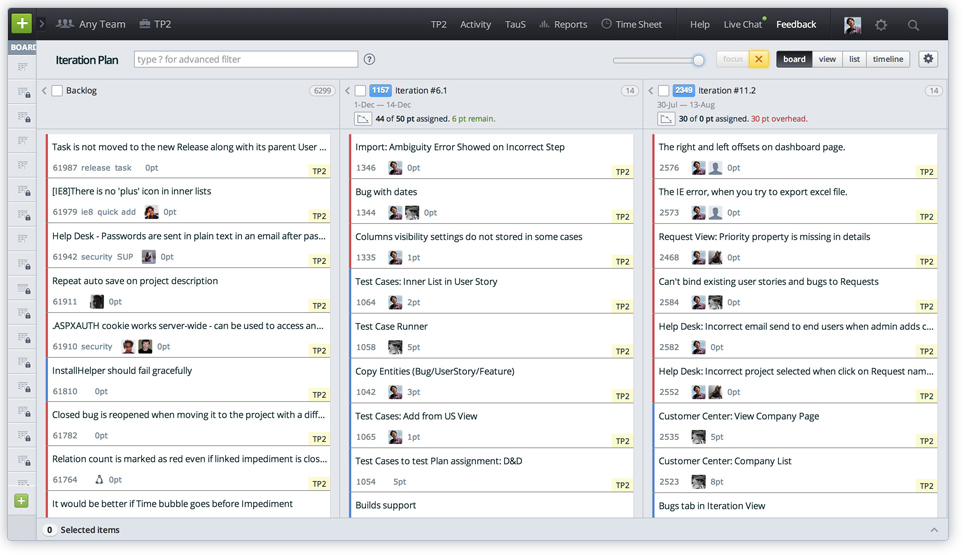
\includegraphics[width=11cm]{preliminaryStudies/targetp.png}
	\caption{TargetProcess's board}
	\label{img:targetp}
\end{figure}

%%%%%%%%%%%%%%%%%%%%%%%%%%%%%%%%%%%%%%%%%%%%%%%%%%%%%%%%%%%%%%%%%%%%%%%%%%%%%%%%%%%%%%%%%%%%%%%%%%%%
%%%%%%%%%%%%%%%%%%%%%%%%%%%%%%%%%%%%%%%%%%%%%%%%%%%%%%%%%%%%%%%%%%%%%%%%%%%%%%%%%%%%%%%%%%%%%%%%%%%%

\section{Version control tools}
Version control systems (VCS) are usually stand-alone applications but they can be integrated into other applications. These system usually allow users to browse previous versions of content. We have decided that we will use VCS both for source code of applications and for project report. 

As every member of the team had experience with different version control systems, they become our candidates. As our team works both on Microsoft Windows and GNU/Linux, it is necessary that chosen VCS supports clients in both platforms. Another criteria was support of online code repository free of charge.

%==================================================================================================%

\subsection{Subversion}
Subversion or SVN is an open source centralized VCS and has many clients across different platforms. 
SVN is supported by Google Code\footnote{\url{http://code.google.com/}} repository.
SVN supports atomic commits, branching and more. Although this tool provides the user with all of the necessary functionality we decided not to use it as the customer suggested to use the other tool.

%==================================================================================================%

\subsection{Git}
Git on the other hand is distributed VCS and offers immediate offline operations.
Projects like Linux kernel\footnote{\url{https://www.kernel.org/}} and Glibc\footnote{\url{https://www.gnu.org/software/libc/}} are using Git as a VCS.
Although Git was created by Linus Torvalds, there are Windows clients available.
Git is supported by GitHub\footnote{\url{https://github.com/}}, what is web-based hosting service for VCS. We have adopted Git as our version control system due to our customer suggestion, the distribution feature and our good experience with Github.
You can find our repository on \url{https://github.com/dohnto/CDP} page.

\begin{figure}[!t]
	\centering
		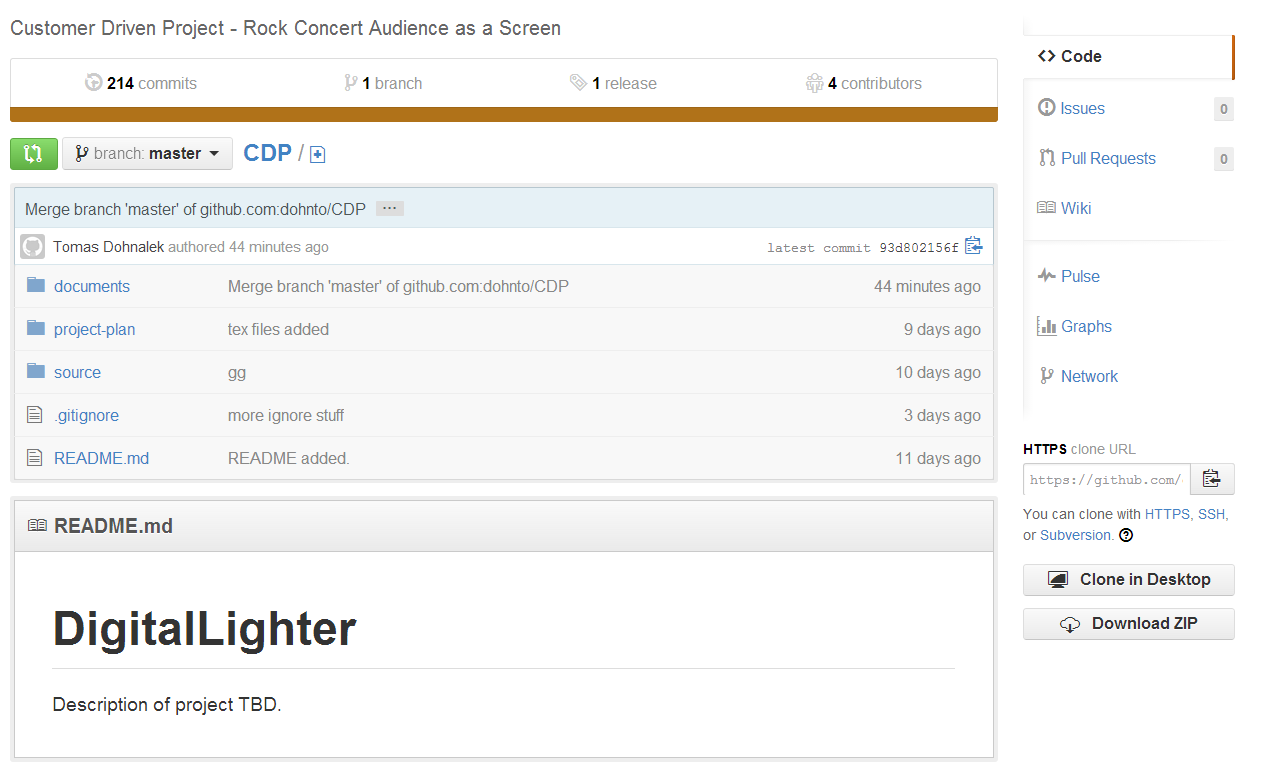
\includegraphics[width=10cm]{preliminaryStudies/git.png}
	\caption{Our github page}
	\label{img:git}
\end{figure}


%%%%%%%%%%%%%%%%%%%%%%%%%%%%%%%%%%%%%%%%%%%%%%%%%%%%%%%%%%%%%%%%%%%%%%%%%%%%%%%%%%%%%%%%%%%%%%%%%%%%
%%%%%%%%%%%%%%%%%%%%%%%%%%%%%%%%%%%%%%%%%%%%%%%%%%%%%%%%%%%%%%%%%%%%%%%%%%%%%%%%%%%%%%%%%%%%%%%%%%%%

\section{Communication tools} \label{txt:communication tools}
Regular Communication with stakeholders and creation of a positive understanding is one of the essential parts of the successful project that can help build effective long-term relationships all parties benefit from. Not only the development team should meet the customer and the supervisor on regular basis but there is also the need for easy distribution and sharing of all kind of the documents. As the time resources of all parties are limited the right collaboration tools enabling seamless and fast communication must be established.

There are certain standard tools that are widely used as a mean of exchanging both textual information and data files. The mainstream well known and effective tools include standard e-mail for messaging, tool for video conferencing, cloud system for data sharing and/or calendar for planning the meetings. Certain platforms providing all necessary tools exist, one can choose among solutions made by Microsoft, Apple, Google and Facebook to list a few most popular.

%==================================================================================================%

\subsection{Email}
Standard email messages will serve the purpose of the communication mean.

%==================================================================================================%

\subsection{Google Drive}
In order to provide the customer with the convenient overview of the work done all relevant documents including the meeting minutes, private notes taken during the meetings and the project report are stored on the Google drive cloud storage service and shared with the customer.

%==================================================================================================%

\subsection{Google Calendar}
The shared Google Calendar was established to keep track of arranged meetings.

%==================================================================================================%

\subsection{Skype}
The Skype is used as a videoconferencing tool as it is considered to be a software of a good quality and the customer disposes of the Skype account.

%==================================================================================================%

\subsection{Facebook group}
For the purpose of internal communication and data exchange among the team members a Facebook group was chosen.

%%%%%%%%%%%%%%%%%%%%%%%%%%%%%%%%%%%%%%%%%%%%%%%%%%%%%%%%%%%%%%%%%%%%%%%%%%%%%%%%%%%%%%%%%%%%%%%%%%%%
%%%%%%%%%%%%%%%%%%%%%%%%%%%%%%%%%%%%%%%%%%%%%%%%%%%%%%%%%%%%%%%%%%%%%%%%%%%%%%%%%%%%%%%%%%%%%%%%%%%%

\section{Documentation tools} \label{txt:documentation tools}

There are basically two options for documentation writing. It is either possible to use WYSIWYG editor such as Microsoft Word, Libre Office or document preparation system based on markup language such as \LaTeX.

\subsection{LaTeX}

It was strongly suggested by the customer to use the latter one as the reports written using \LaTeX  tend to make more professional impression.


